\begin{figure}[tbp]
\centering
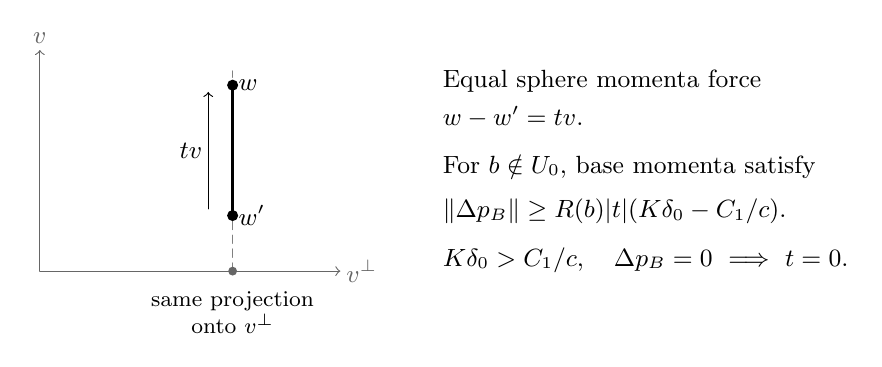
\begin{tikzpicture}[x=0.72cm,y=0.72cm,font=\small,
  every node/.style={inner sep=2pt},line cap=round]
  \draw[->,black!60] (0,0.5)--(5.3,0.5) node[right] {$v^\perp$};
  \draw[->,black!60] (0,0.5)--(0,4.4) node[above] {$v$};
  \draw[densely dashed,black!50] (3.4,0.5)--(3.4,4.03);
  \draw[line width=1pt] (3.4,1.48)--(3.4,3.78);
  \fill (3.4,1.48) circle (2pt) node[right] {$w'$};
  \fill (3.4,3.78) circle (2pt) node[right] {$w$};
  \draw[->] (2.97,1.6)--(2.97,3.66)
    node[midway,left] {$tv$};
  \fill[black!60] (3.4,0.5) circle (1.6pt);
  \node[anchor=north,align=center,font=\footnotesize] at (3.4,0.24)
    {same projection\\onto $v^\perp$};
  \node[anchor=west] at (7,3.85) {Equal sphere momenta force};
  \node[anchor=west] at (7,3.22) {$w-w'=tv$.};
  \node[anchor=west] at (7,2.35) {For $b\notin U_0$, base momenta satisfy};
  \node[anchor=west] at (7,1.55)
    {$\|\Delta p_B\|\geq R(b)|t|(K\delta_0-C_1/c)$.};
  \node[anchor=west] at (7,0.7)
    {$K\delta_0>C_1/c,\quad \Delta p_B=0\ \Longrightarrow\ t=0$.};
\end{tikzpicture}
\caption{Schematic of the two momentum tests for two critical points at
fixed base coordinates $(b,v)$, with $\Delta p_B$ the difference of the $B$-momenta. Sphere
momenta detect the component of $w$ perpendicular to $v$; the varying
scale separates the remaining pairs outside $U_0$.
Within $U_0$, the fixed quadratic critical equation has a unique solution.
The two-dimensional drawing represents an orthogonal decomposition only.
The estimate also holds when the segment from $w'$ to $w$ passes through
zero.}
\label{fig:momentum-separation}
\end{figure}
